% General match
\DeclareMathOperator*{\argmax}{arg\,max}
\DeclareMathOperator*{\argmin}{arg\,min}
\newcommand{\mli}[1]{\mathit{#1}}
\newcommand{\concat}[0]{{\cdot}}
%\newcommand{\bp}{\,bp} %\newcommand{\bp}{\unit{\,bp}}
%\newcommand{\kbp}{\,kbp} %\newcommand{\kbp}{\unit{\,kbp}}
\newcommand{\qty}[2]{#1\ #2} % TODO: remove \qty and \unit in favor of siunitx
\newcommand{\unit}[1]{#1} 
\newcommand{\Oh}[0]{O}
\newcommand{\ed}[0]{\mbox{ed}\xspace}
\newcommand{\st}[2]{\langle #1, #2 \rangle}

% Edit costs
\newcommand{\Costs}[0]{\mathbb{R}_{\geq 0}}
\newcommand{\costcap}[0]{c}
\newcommand{\cedits}[0]{\Delta}
\newcommand{\cmatch}[0]{\Delta_\text{match}}
\newcommand{\csubst}[0]{\Delta_\text{subst}}
\newcommand{\cins}[0]{\Delta_\text{ins}}
\newcommand{\cdel}[0]{\Delta_\text{del}}
\newcommand{\dist}[0]{\mli{ED_\Delta}}
\newcommand{\maxdel}[0]{n_\text{del}}
\newcommand{\maxins}[0]{n_\text{ins}}

% Graph terms
\newcommand{\g}{g^*\!}
\newcommand{\h}{h^*\!}
\newcommand{\A}[0]{A$^\star$\xspace}
\newcommand{\Path}{\pi^*}
% reference graph
\newcommand{\reference}[1]{#1_\texttt{r}}
\newcommand{\RG}[0]{\reference{G}}
\newcommand{\RGV}[0]{\reference{V}}
\newcommand{\RGE}[0]{\reference{E}}
% trie
\newcommand{\trie}[1]{#1_\texttt{r}^\texttt{+}}
\newcommand{\TG}[0]{\trie{G}}
\newcommand{\TGV}[0]{\trie{V}}
\newcommand{\TGE}[0]{\trie{E}}

% edit graph; depracated: use \AG
%\newcommand{\edit}[1]{#1_\texttt{e}}
%\newcommand{\EG}[0]{\edit{G}}
%\newcommand{\EGV}[0]{\edit{V}}
%\newcommand{\EGE}[0]{\edit{E}}

% alignment graph
% TODO: simplify to just G(V,E)
%\newcommand{\alignment}[2][q]{#2_\texttt{a}^{#1}}
\newcommand{\alignment}[2][q]{#2}
\newcommand{\AG}[1][q]{\alignment[#1]{G}}
\newcommand{\AGV}[1][q]{\alignment[#1]{V}}
\newcommand{\AGE}[1][q]{\alignment[#1]{E}}

% Seed heuristic
%\newcommand{\csh}[0]{chaining seed heuristic\xspace}
%\newcommand{\Csh}[0]{Chaining seed heuristic\xspace}
%\newcommand{\CSH}[0]{CSH\xspace}
%\newcommand{\sh}[0]{seed heuristic\xspace}
%\newcommand{\Sh}[0]{Seed heuristic\xspace}
%\newcommand{\SH}[0]{SH\xspace}
%\newcommand{\seeds}{\mathcal S}
%\newcommand{\matches}{\mathcal M}
%\newcommand{\Pot}{P}
%\newcommand{\spot}{r}
\newcommand{\cost}{\operatorname{cost}}
%\newcommand{\matchscore}{\operatorname{score}}
%\newcommand{\seedscore}{\operatorname{score}}
%\newcommand{\statescore}{S}
%\newcommand{\chainscore}{S_{\mathrm{chain}}}
%\newcommand{\shscore}{S_{\mathrm{sh}}}
%\newcommand{\cshscore}{S_{\mathrm{csh}}}

%\newcommand{\seedh}[0]{\mbox{seed heuristic}\xspace}
\newcommand{\prefixh}[0]{\mbox{prefix heuristic}\xspace}
\newcommand{\trieroot}{\ensuremath{\mli{root}}}

%% Global alignment
%% Fig.2
%\newcommand{\bluecircle}{
\includegraphics[height=4pt]{paper-global/imgs/fig2-symbols/blue-circle.pdf}}
%\newcommand{\greencircle}{
\includegraphics[height=4pt]{paper-global/imgs/fig2-symbols/green-circle.pdf}}
%\newcommand{\cross}{
\includegraphics[height=4pt]{paper-global/imgs/fig2-symbols/cross.pdf}}
%\newcommand{\seed}{
\includegraphics[width=6pt]{paper-global/imgs/fig2-symbols/seed.pdf}}
%\newcommand{\match}{
\includegraphics[height=4pt]{paper-global/imgs/fig2-symbols/match.pdf}}
%\newcommand{\redcolumn}{
\includegraphics[height=5pt]{paper-global/imgs/fig2-symbols/red-column.pdf}}
%\newcommand{\greencolumn}{
\includegraphics[height=5pt]{paper-global/imgs/fig2-symbols/green-column.pdf}}
%% Fig.3
%\newcommand{\bluesquare}{
\includegraphics[height=4pt]{paper-global/imgs/fig3-symbols/bluesquare.pdf}}
%\newcommand{\greensquare}{
\includegraphics[height=4pt]{paper-global/imgs/fig3-symbols/greensquare.pdf}}
%\newcommand{\blackmatch}{
\includegraphics[height=5pt]{paper-global/imgs/fig3-symbols/blackmatch.pdf}}
%\newcommand{\redmatch}{
\includegraphics[height=5pt]{paper-global/imgs/fig3-symbols/redmatch.pdf}}
%% Plots
%\newcommand{\edlibsymbol}{
\includegraphics[height=4pt]{paper-global/imgs/plots-symbols/edlib.pdf}}
%\newcommand{\wfasymbol}{
\includegraphics[height=4pt]{paper-global/imgs/plots-symbols/wfa.pdf}}
%\newcommand{\shsymbol}{
\includegraphics[height=4pt]{paper-global/imgs/plots-symbols/sh.pdf}}
%\newcommand{\shsymbolsq}{
\includegraphics[height=4pt]{paper-global/imgs/plots-symbols/sh-down.pdf}}
%\newcommand{\cshsymbol}{
\includegraphics[height=4pt]{paper-global/imgs/plots-symbols/csh.pdf}}
%\newcommand{\cshsymbolsq}{
\includegraphics[height=4pt]{paper-global/imgs/plots-symbols/csh-down.pdf}}

% Seeds paper
% crumbs icons
\newcommand{\bluecrumb}{%
  \begingroup\normalfont
  \includegraphics[height=\fontcharht\font`\B]{paper-seed/figures/blue-square.pdf}%
  \endgroup
}
\newcommand{\greencrumb}{%
  \begingroup\normalfont
  
\includegraphics[height=1.1\fontcharht\font`\B]{paper-seed/figures/green-square.pdf}%
  \endgroup
}
\newcommand{\yellowcrumb}{%
  \begingroup\normalfont
  
\includegraphics[height=1.1\fontcharht\font`\B]{paper-seed/figures/yellow-triangle.pdf}%
  \endgroup
}
\newcommand{\violetcrumb}{%
  \begingroup\normalfont
  
\includegraphics[height=\fontcharht\font`\B]{paper-seed/figures/violet-circle.pdf}%
  \endgroup
}
% other icons
\newcommand{\greentick}{%
  \begingroup\normalfont
  
\includegraphics[height=\fontcharht\font`\B]{paper-seed/figures/green-tick.pdf}%
  \endgroup
}

% tools
\newcommand{\dijkstra}[0]{\mbox{Dijkstra}\xspace}
\newcommand{\astarix}[0]{\mbox{\textsc{AStarix}}\xspace}
\newcommand{\astarixseeds}[0]{\mbox{\textsc{AStarix-seeds}}\xspace}
\newcommand{\astarixprefix}[0]{\mbox{\textsc{AStarix-prefix}}\xspace}
\newcommand{\astarixurl}[0]{\url{https://github.com/eth-sri/astarix}\xspace}
\newcommand{\astarixurlwithbranch}[0]{\url{https://github.com/eth-sri/astarix/tree/recomb2020}\xspace}
\newcommand{\graphaligner}[0]{\textsc{GraphAligner}\xspace}
\newcommand{\bitparallel}[0]{\textsc{BitParallel}\xspace}
\newcommand{\brownie}[0]{\textsc{Brownie}\xspace}
\newcommand{\pasgal}[0]{\textsc{PaSGAL}\xspace}
\newcommand{\vg}[0]{\textsc{VG}\xspace}
\newcommand{\valigntool}[0]{\textsc{V-ALIGN}\xspace}
\newcommand{\vargas}[0]{\mbox{\textsc{Vargas}}\xspace}
\newcommand{\hga}[0]{\mbox{\textsc{HGA}}\xspace}
\newcommand{\art}[0]{\mbox{\textsc{ART}}\xspace}
\newcommand{\randomreads}[0]{\mbox{\textsc{randomreads.sh}}\xspace}

% Global alignment tools
%\newcommand{\difftool}[0]{\mbox{\textsc{diff}}\xspace}
%\newcommand{\edlib}[0]{\mbox{\textsc{Edlib}}\xspace}
%\newcommand{\oldwfa}[0]{\mbox{\textsc{WFA}}\xspace}
%\newcommand{\wfa}[0]{\mbox{\textsc{BiWFA}}\xspace}
%\newcommand{\seqan}[0]{\mbox{\textsc{SeqAn}}\xspace}
%\newcommand{\parasail}[0]{\mbox{\textsc{Parasail}}\xspace}
%\newcommand{\astarpa}[0]{\mbox{\textsc{A*PA}}\xspace}
%\newcommand{\lcs}[0]{\mbox{LCS}\xspace}
%\newcommand{\lcskpp}[0]{\mbox{LCSk++}\xspace}

% Datasets
\newcommand{\datasetOne}{CHM13}
\newcommand{\datasetTwo}{NA12878}

% paper-global

\makeatletter
\newcommand\nopagebreaklist{\par\nobreak\@afterheading}
\makeatother

%\newcommand{\A}[0]{A\!$^\star$\xspace}
%\newcommand{\A}[0]{A*\xspace}
\newcommand{\sh}[0]{seed heuristic\xspace}
\newcommand{\Sh}[0]{Seed heuristic\xspace}
\newcommand{\SH}[0]{SH\xspace}
\newcommand{\csh}[0]{chaining seed heuristic\xspace}
\newcommand{\Csh}[0]{Chaining seed heuristic\xspace}
\newcommand{\CSH}[0]{CSH\xspace}
\newcommand{\gch}[0]{gap-chaining seed heuristic\xspace}
\newcommand{\Gch}[0]{Gap-chaining seed heuristic\xspace}
\newcommand{\GCH}[0]{GCSH\xspace}
\newcommand{\wah}[0]{weakly-admissible heuristic\xspace}
\newcommand{\Wah}[0]{Weakly-admissible heuristic\xspace}
\newcommand{\wa}[0]{weakly admissible\xspace}
\newcommand{\Wa}[0]{Weakly admissible\xspace}
\newcommand{\way}[0]{weak admissibility\xspace}
%\newcommand{\mpp}[0]{multiple-path pruning\xspace}
%\newcommand{\Mpp}[0]{Multiple-path pruning\xspace}

\newcommand{\lcs}[0]{\mbox{LCS}\xspace}
\newcommand{\lcskpp}[0]{\mbox{LCSk++}\xspace}
\newcommand{\pa}[0]{pairwise alignment\xspace}
%\newcommand{\ed}{\operatorname{ed}}
\renewcommand{\d}{\operatorname{d}}

% tool names
\newcommand{\difftool}[0]{\mbox{\textsc{diff}}\xspace}
\newcommand{\edlib}[0]{\mbox{\textsc{Edlib}}\xspace}
\newcommand{\oldwfa}[0]{\mbox{\textsc{WFA}}\xspace}
\newcommand{\wfa}[0]{\mbox{\textsc{BiWFA}}\xspace}
\newcommand{\seqan}[0]{\mbox{\textsc{SeqAn}}\xspace}
\newcommand{\parasail}[0]{\mbox{\textsc{Parasail}}\xspace}
\newcommand{\astarpa}[0]{\mbox{\textsc{A*PA}}\xspace}
%\newcommand{\astarix}[0]{\mbox{\textsc{AStarix}}\xspace}
%\newcommand{\dijkstra}[0]{\mbox{Dijkstra}\xspace}
\newcommand{\pabench}[0]{\mbox{\textsc{PaBench}}\xspace}
\newcommand{\DT}[0]{DT\xspace}

\titleformat{\paragraph}[runin]{\normalfont\bfseries\boldmath}{}{}{\hspace{\parindent}}[.]
\titlespacing*{\paragraph}{0pt}{0pt}{0.5em}

\setlength{\abovecaptionskip}{5pt plus 0pt minus 0pt}

% general math
\newcommand{\seeds}{\mathcal S}
\newcommand{\matches}{\mathcal M}
\newcommand{\Expanded}{E}
\newcommand{\prunedmatches}{{\matches\backslash\Expanded}}

% Algorithm stages
%\newcommand{\algletter}{ALGLETTER}
%\newcommand{\stageAstar}{A\!$^\star$}
%\newcommand{\stageDT}{DT}
%\newcommand{\stagePrecomp}{Pre}
%\newcommand{\stageHeuristic}{H}
%\newcommand{\stagePrune}{Prune}

% Commands for A* functions
%\newcommand{\st}[2]{\langle #1, #2 \rangle}
%\newcommand{\g}{g^*\!}
%\newcommand{\h}{h^*\!}
\newcommand{\ssh}{_{\mathrm{s}}}
\newcommand{\scsh}{_{\mathrm{cs}}}
\newcommand{\sgch}{_{\mathrm{gcs}}}
\newcommand{\hsh}{h\ssh\!}
\newcommand{\hcsh}{h\scsh\!}
\newcommand{\hgch}{h\sgch\!}
\newcommand{\hM}{h^\matches\!}
\newcommand{\hshM}{h\ssh^\matches\!}
\newcommand{\hcshM}{h\scsh^\matches\!}
\newcommand{\hgchM}{h\sgch^\matches\!}
\newcommand{\hh}{\hat h}
\newcommand{\hshS}{\hat h\ssh\!}
\newcommand{\hcshS}{\hat h\scsh\!}
\newcommand{\hgchS}{\hat h\sgch\!}
%% \newcommand{\hshSM}{\hat h\ssh^\matches\!}
%% \newcommand{\hcshSM}{\hat h\scsh^\matches\!}
%% \newcommand{\hgchSM}{\hat h\sgch^\matches\!}
%\newcommand{\Path}{\pi^*}

% DT
\newcommand{\DTA}{DT-\A}
%\newcommand{\fr}{\mathcal F}
\newcommand{\LCP}{\operatorname{LCP}}
\newcommand{\dst}[2]{\llangle #1, #2 \rrangle}
%\newcommand{\wt}{\widetilde}
\newcommand{\wt}{}
\newcommand{\fr}{F}
\newcommand{\x}{X}
\newcommand{\du}{\wt u}
\newcommand{\dv}{\wt v}

% Functions
\newcommand{\Pot}{P}
\newcommand{\spot}{r}
\newcommand{\matchcost}{\operatorname{c_{\mathrm{m}}}}
\newcommand{\pathcost}{\operatorname{c_{\mathrm{path}}}}
\newcommand{\matchscore}{\operatorname{score}}
\newcommand{\seedscore}{\operatorname{score}}
\newcommand{\statescore}{S}
\newcommand{\chainscore}{S_{\mathrm{chain}}}
\newcommand{\shscore}{S_{\mathrm{s}}}
\newcommand{\cshscore}{S_{\mathrm{cs}}}

\newcommand{\layer}{\mathcal L}
\newcommand{\start}{\operatorname{start}}
\newcommand{\substr}[3]{#1_{#2{\dots}#3}}
\newcommand{\abs}[1]{\lvert #1 \rvert}

% Gapcost
\newcommand{\gapcost}{c_{\mathrm{gap}}}
\newcommand{\seedcost}{c_{\mathrm{seed}}}
\newcommand{\gscost}{c_{\mathrm{gs}}}
\newcommand{\gchscore}{S_{\mathrm{gchs}}}
% transformation
\newcommand{\T}{T}
\newcommand{\preceqsq}{\sqsubseteq}
\newcommand{\npreceqsq}{\nsqsubseteq}
\newcommand{\precsq}{\sqsubset}
\newcommand{\nprecsq}{\nsqsubset}
%\newcommand{\tst}[2]{\llbracket #1, #2\rrbracket}
\newcommand{\tst}[2]{( #1, #2)}
\newcommand{\matchstart}{\operatorname{start}}
\newcommand{\matchend}{\operatorname{end}}

% Fig.2
\newcommand{\bluecircle}{
\includegraphics[height=4pt]{paper-global/imgs/heuristic-diagrams-symbols/blue-circle.pdf}}
\newcommand{\greencircle}{
\includegraphics[height=4pt]{paper-global/imgs/heuristic-diagrams-symbols/green-circle.pdf}}
\newcommand{\cross}{
\includegraphics[height=4pt]{paper-global/imgs/heuristic-diagrams-symbols/cross.pdf}}
\newcommand{\seed}{
\includegraphics[width=6pt]{paper-global/imgs/heuristic-diagrams-symbols/seed.pdf}}
\newcommand{\match}{
\includegraphics[height=4pt]{paper-global/imgs/heuristic-diagrams-symbols/match.pdf}}
\newcommand{\redcolumn}{
\includegraphics[height=5pt]{paper-global/imgs/heuristic-diagrams-symbols/red-column.pdf}}
\newcommand{\greencolumn}{
\includegraphics[height=5pt]{paper-global/imgs/heuristic-diagrams-symbols/green-column.pdf}}

% Fig.3
\newcommand{\bluesquare}{
\includegraphics[height=4pt]{paper-global/imgs/layers-symbols/bluesquare.pdf}}
\newcommand{\greensquare}{
\includegraphics[height=4pt]{paper-global/imgs/layers-symbols/greensquare.pdf}}
\newcommand{\blackmatch}{
\includegraphics[height=5pt]{paper-global/imgs/layers-symbols/blackmatch.pdf}}
\newcommand{\redmatch}{
\includegraphics[height=5pt]{paper-global/imgs/layers-symbols/redmatch.pdf}}

% Plots
% \newcommand{\edlibsymbol}{
\includegraphics[height=4pt]{imgs/plots-symbols/edlib.pdf}}
% \newcommand{\wfasymbol}{
\includegraphics[height=4pt]{imgs/plots-symbols/wfa.pdf}}
% \newcommand{\shsymbol}{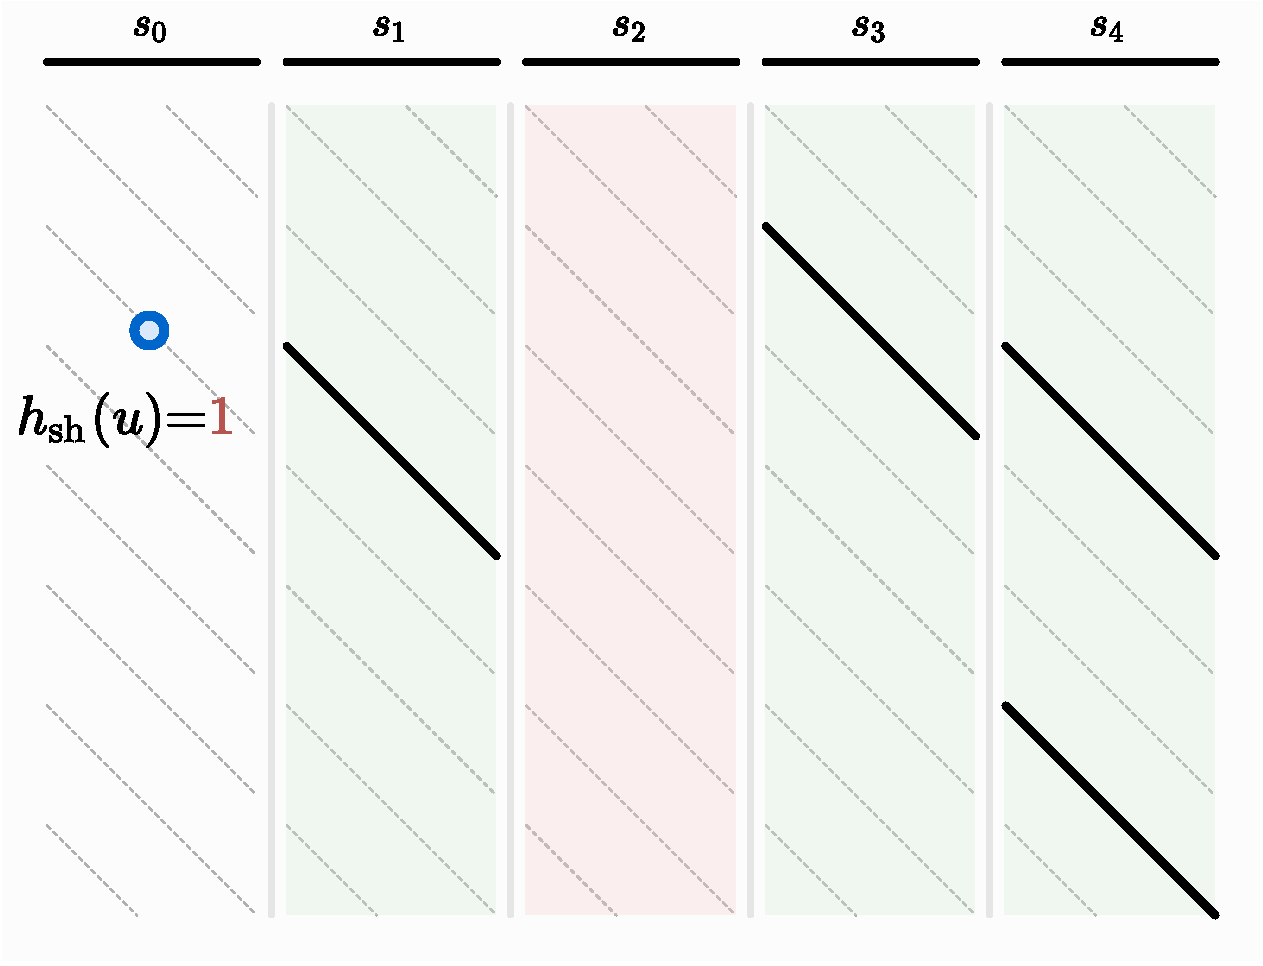
\includegraphics[height=4pt]{imgs/plots-symbols/sh.pdf}}
% \newcommand{\shsymbolsq}{
\includegraphics[height=4pt]{imgs/plots-symbols/sh-down.pdf}}
% \newcommand{\cshsymbol}{
\includegraphics[height=4pt]{imgs/plots-symbols/csh.pdf}}
% \newcommand{\cshsymbolsq}{
\includegraphics[height=4pt]{imgs/plots-symbols/csh-down.pdf}}

% Units
\newcommand{\bp}{\unit{\,bp}}
\newcommand{\kbp}{\unit{\,kbp}}
\newcommand{\mb}{\unit{\,MB}}
